% Created by tikzDevice version 0.12.3.2 on 2022-02-15 15:54:04
% !TEX encoding = UTF-8 Unicode
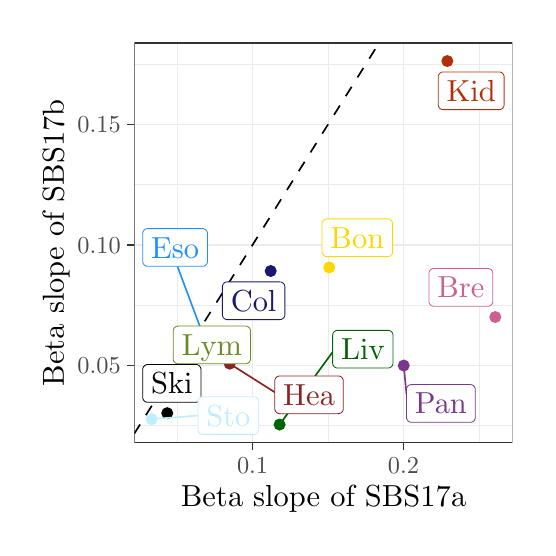
\begin{tikzpicture}[x=1pt,y=1pt]
\definecolor{fillColor}{RGB}{255,255,255}
\path[use as bounding box,fill=fillColor,fill opacity=0.00] (0,0) rectangle (180.67,180.67);
\begin{scope}
\path[clip] (  0.00,  0.00) rectangle (180.67,180.67);
\definecolor{drawColor}{RGB}{255,255,255}
\definecolor{fillColor}{RGB}{255,255,255}

\path[draw=drawColor,line width= 0.6pt,line join=round,line cap=round,fill=fillColor] (  0.00,  0.00) rectangle (180.68,180.68);
\end{scope}
\begin{scope}
\path[clip] ( 38.56, 30.69) rectangle (175.17,175.17);
\definecolor{fillColor}{RGB}{255,255,255}

\path[fill=fillColor] ( 38.56, 30.69) rectangle (175.18,175.17);
\definecolor{drawColor}{gray}{0.92}

\path[draw=drawColor,line width= 0.3pt,line join=round] ( 38.56, 36.89) --
	(175.17, 36.89);

\path[draw=drawColor,line width= 0.3pt,line join=round] ( 38.56, 80.42) --
	(175.17, 80.42);

\path[draw=drawColor,line width= 0.3pt,line join=round] ( 38.56,123.96) --
	(175.17,123.96);

\path[draw=drawColor,line width= 0.3pt,line join=round] ( 38.56,167.49) --
	(175.17,167.49);

\path[draw=drawColor,line width= 0.3pt,line join=round] ( 53.99, 30.69) --
	( 53.99,175.17);

\path[draw=drawColor,line width= 0.3pt,line join=round] (108.54, 30.69) --
	(108.54,175.17);

\path[draw=drawColor,line width= 0.3pt,line join=round] (163.09, 30.69) --
	(163.09,175.17);

\path[draw=drawColor,line width= 0.6pt,line join=round] ( 38.56, 58.65) --
	(175.17, 58.65);

\path[draw=drawColor,line width= 0.6pt,line join=round] ( 38.56,102.19) --
	(175.17,102.19);

\path[draw=drawColor,line width= 0.6pt,line join=round] ( 38.56,145.72) --
	(175.17,145.72);

\path[draw=drawColor,line width= 0.6pt,line join=round] ( 81.27, 30.69) --
	( 81.27,175.17);

\path[draw=drawColor,line width= 0.6pt,line join=round] (135.81, 30.69) --
	(135.81,175.17);
\definecolor{drawColor}{RGB}{0,0,0}

\path[draw=drawColor,line width= 0.6pt,dash pattern=on 4pt off 4pt ,line join=round] ( 17.25,  0.00) -- (130.44,180.67);
\definecolor{drawColor}{RGB}{255,215,0}
\definecolor{fillColor}{RGB}{255,215,0}

\path[draw=drawColor,line width= 0.4pt,line join=round,line cap=round,fill=fillColor] (108.98, 94.03) circle (  1.96);
\definecolor{drawColor}{RGB}{205,96,144}
\definecolor{fillColor}{RGB}{205,96,144}

\path[draw=drawColor,line width= 0.4pt,line join=round,line cap=round,fill=fillColor] (168.97, 76.10) circle (  1.96);
\definecolor{drawColor}{RGB}{25,25,112}
\definecolor{fillColor}{RGB}{25,25,112}

\path[draw=drawColor,line width= 0.4pt,line join=round,line cap=round,fill=fillColor] ( 87.81, 92.74) circle (  1.96);
\definecolor{drawColor}{RGB}{30,144,255}
\definecolor{fillColor}{RGB}{30,144,255}

\path[draw=drawColor,line width= 0.4pt,line join=round,line cap=round,fill=fillColor] ( 63.59, 69.09) circle (  1.96);
\definecolor{drawColor}{RGB}{139,35,35}
\definecolor{fillColor}{RGB}{139,35,35}

\path[draw=drawColor,line width= 0.4pt,line join=round,line cap=round,fill=fillColor] ( 73.01, 59.25) circle (  1.96);
\definecolor{drawColor}{RGB}{179,47,11}
\definecolor{fillColor}{RGB}{179,47,11}

\path[draw=drawColor,line width= 0.4pt,line join=round,line cap=round,fill=fillColor] (151.64,168.61) circle (  1.96);
\definecolor{drawColor}{RGB}{0,100,0}
\definecolor{fillColor}{RGB}{0,100,0}

\path[draw=drawColor,line width= 0.4pt,line join=round,line cap=round,fill=fillColor] ( 91.03, 37.25) circle (  1.96);
\definecolor{drawColor}{RGB}{105,139,34}
\definecolor{fillColor}{RGB}{105,139,34}

\path[draw=drawColor,line width= 0.4pt,line join=round,line cap=round,fill=fillColor] ( 70.23, 63.41) circle (  1.96);
\definecolor{drawColor}{RGB}{122,55,139}
\definecolor{fillColor}{RGB}{122,55,139}

\path[draw=drawColor,line width= 0.4pt,line join=round,line cap=round,fill=fillColor] (135.89, 58.59) circle (  1.96);
\definecolor{drawColor}{RGB}{0,0,0}
\definecolor{fillColor}{RGB}{0,0,0}

\path[draw=drawColor,line width= 0.4pt,line join=round,line cap=round,fill=fillColor] ( 50.43, 41.37) circle (  1.96);
\definecolor{drawColor}{RGB}{191,239,255}
\definecolor{fillColor}{RGB}{191,239,255}

\path[draw=drawColor,line width= 0.4pt,line join=round,line cap=round,fill=fillColor] ( 44.77, 39.20) circle (  1.96);
\end{scope}
\begin{scope}
\path[clip] ( 38.56, 30.69) rectangle (175.17,175.17);
\definecolor{drawColor}{RGB}{30,144,255}

\path[draw=drawColor,line width= 0.6pt,line join=round,line cap=round] ( 54.11, 94.43) -- ( 63.27, 69.95);
\definecolor{drawColor}{RGB}{139,35,35}

\path[draw=drawColor,line width= 0.6pt,line join=round,line cap=round] ( 89.31, 48.92) -- ( 73.76, 58.77);
\definecolor{drawColor}{RGB}{0,100,0}

\path[draw=drawColor,line width= 0.6pt,line join=round,line cap=round] (110.19, 63.45) -- ( 91.57, 37.99);
\definecolor{drawColor}{RGB}{122,55,139}

\path[draw=drawColor,line width= 0.6pt,line join=round,line cap=round] (136.87, 48.24) -- (135.98, 57.67);
\definecolor{drawColor}{RGB}{191,239,255}

\path[draw=drawColor,line width= 0.6pt,line join=round,line cap=round] ( 61.52, 40.51) -- ( 45.64, 39.27);
\definecolor{drawColor}{RGB}{255,215,0}
\definecolor{fillColor}{RGB}{255,255,255}

\path[draw=drawColor,line width= 0.3pt,line join=round,line cap=round,fill=fillColor] (108.18, 97.94) --
	(130.06, 97.94) --
	(129.99, 97.94) --
	(130.28, 97.96) --
	(130.56, 98.01) --
	(130.84, 98.12) --
	(131.09, 98.26) --
	(131.31, 98.45) --
	(131.51, 98.66) --
	(131.66, 98.91) --
	(131.77, 99.18) --
	(131.84, 99.46) --
	(131.87, 99.75) --
	(131.87, 99.75) --
	(131.87,109.76) --
	(131.87,109.76) --
	(131.84,110.05) --
	(131.77,110.33) --
	(131.66,110.60) --
	(131.51,110.85) --
	(131.31,111.06) --
	(131.09,111.25) --
	(130.84,111.39) --
	(130.56,111.50) --
	(130.28,111.56) --
	(130.06,111.57) --
	(108.18,111.57) --
	(108.40,111.56) --
	(108.11,111.57) --
	(107.82,111.53) --
	(107.54,111.45) --
	(107.28,111.33) --
	(107.04,111.16) --
	(106.83,110.96) --
	(106.66,110.73) --
	(106.52,110.47) --
	(106.43,110.19) --
	(106.38,109.91) --
	(106.38,109.76) --
	(106.38, 99.75) --
	(106.38, 99.89) --
	(106.38, 99.60) --
	(106.43, 99.32) --
	(106.52, 99.04) --
	(106.66, 98.78) --
	(106.83, 98.55) --
	(107.04, 98.35) --
	(107.28, 98.18) --
	(107.54, 98.06) --
	(107.82, 97.98) --
	(108.11, 97.94) --
	cycle;
\end{scope}
\begin{scope}
\path[clip] ( 38.56, 30.69) rectangle (175.17,175.17);
\definecolor{drawColor}{RGB}{255,215,0}

\node[text=drawColor,anchor=base,inner sep=0pt, outer sep=0pt, scale=  1.10] at (119.12,100.95) {Bon};
\definecolor{drawColor}{RGB}{205,96,144}
\definecolor{fillColor}{RGB}{255,255,255}

\path[draw=drawColor,line width= 0.3pt,line join=round,line cap=round,fill=fillColor] (146.81, 80.01) --
	(166.26, 80.01) --
	(166.19, 80.01) --
	(166.48, 80.02) --
	(166.76, 80.08) --
	(167.04, 80.18) --
	(167.29, 80.33) --
	(167.51, 80.51) --
	(167.71, 80.73) --
	(167.86, 80.98) --
	(167.98, 81.24) --
	(168.04, 81.53) --
	(168.07, 81.82) --
	(168.07, 81.82) --
	(168.07, 91.83) --
	(168.07, 91.83) --
	(168.04, 92.12) --
	(167.98, 92.40) --
	(167.86, 92.67) --
	(167.71, 92.91) --
	(167.51, 93.13) --
	(167.29, 93.31) --
	(167.04, 93.46) --
	(166.76, 93.56) --
	(166.48, 93.62) --
	(166.26, 93.63) --
	(146.81, 93.63) --
	(147.02, 93.62) --
	(146.73, 93.63) --
	(146.44, 93.60) --
	(146.17, 93.52) --
	(145.90, 93.39) --
	(145.66, 93.23) --
	(145.45, 93.03) --
	(145.28, 92.79) --
	(145.14, 92.54) --
	(145.05, 92.26) --
	(145.01, 91.97) --
	(145.00, 91.83) --
	(145.00, 81.82) --
	(145.01, 81.96) --
	(145.01, 81.67) --
	(145.05, 81.38) --
	(145.14, 81.11) --
	(145.28, 80.85) --
	(145.45, 80.62) --
	(145.66, 80.42) --
	(145.90, 80.25) --
	(146.17, 80.13) --
	(146.44, 80.05) --
	(146.73, 80.01) --
	cycle;
\end{scope}
\begin{scope}
\path[clip] ( 38.56, 30.69) rectangle (175.17,175.17);
\definecolor{drawColor}{RGB}{205,96,144}

\node[text=drawColor,anchor=base,inner sep=0pt, outer sep=0pt, scale=  1.10] at (156.53, 83.02) {Bre};
\definecolor{drawColor}{RGB}{25,25,112}
\definecolor{fillColor}{RGB}{255,255,255}

\path[draw=drawColor,line width= 0.3pt,line join=round,line cap=round,fill=fillColor] ( 72.16, 75.18) --
	( 91.12, 75.18) --
	( 91.05, 75.18) --
	( 91.34, 75.19) --
	( 91.63, 75.25) --
	( 91.90, 75.35) --
	( 92.15, 75.50) --
	( 92.38, 75.68) --
	( 92.57, 75.90) --
	( 92.72, 76.14) --
	( 92.84, 76.41) --
	( 92.91, 76.69) --
	( 92.93, 76.98) --
	( 92.93, 76.98) --
	( 92.93, 87.00) --
	( 92.93, 87.00) --
	( 92.91, 87.29) --
	( 92.84, 87.57) --
	( 92.72, 87.84) --
	( 92.57, 88.08) --
	( 92.38, 88.30) --
	( 92.15, 88.48) --
	( 91.90, 88.63) --
	( 91.63, 88.73) --
	( 91.34, 88.79) --
	( 91.12, 88.80) --
	( 72.16, 88.80) --
	( 72.38, 88.79) --
	( 72.09, 88.80) --
	( 71.80, 88.77) --
	( 71.52, 88.69) --
	( 71.26, 88.56) --
	( 71.02, 88.40) --
	( 70.81, 88.19) --
	( 70.63, 87.96) --
	( 70.50, 87.70) --
	( 70.41, 87.43) --
	( 70.36, 87.14) --
	( 70.35, 87.00) --
	( 70.35, 76.98) --
	( 70.36, 77.13) --
	( 70.36, 76.84) --
	( 70.41, 76.55) --
	( 70.50, 76.28) --
	( 70.63, 76.02) --
	( 70.81, 75.79) --
	( 71.02, 75.58) --
	( 71.26, 75.42) --
	( 71.52, 75.29) --
	( 71.80, 75.21) --
	( 72.09, 75.18) --
	cycle;
\end{scope}
\begin{scope}
\path[clip] ( 38.56, 30.69) rectangle (175.17,175.17);
\definecolor{drawColor}{RGB}{25,25,112}

\node[text=drawColor,anchor=base,inner sep=0pt, outer sep=0pt, scale=  1.10] at ( 81.64, 78.19) {Col};
\definecolor{drawColor}{RGB}{30,144,255}
\definecolor{fillColor}{RGB}{255,255,255}

\path[draw=drawColor,line width= 0.3pt,line join=round,line cap=round,fill=fillColor] ( 43.37, 94.43) --
	( 63.17, 94.43) --
	( 63.09, 94.43) --
	( 63.38, 94.44) --
	( 63.67, 94.50) --
	( 63.94, 94.60) --
	( 64.19, 94.75) --
	( 64.42, 94.93) --
	( 64.61, 95.15) --
	( 64.77, 95.40) --
	( 64.88, 95.66) --
	( 64.95, 95.95) --
	( 64.97, 96.24) --
	( 64.97, 96.24) --
	( 64.97,106.25) --
	( 64.97,106.25) --
	( 64.95,106.54) --
	( 64.88,106.82) --
	( 64.77,107.09) --
	( 64.61,107.33) --
	( 64.42,107.55) --
	( 64.19,107.74) --
	( 63.94,107.88) --
	( 63.67,107.98) --
	( 63.38,108.04) --
	( 63.17,108.06) --
	( 43.37,108.06) --
	( 43.59,108.04) --
	( 43.30,108.05) --
	( 43.01,108.02) --
	( 42.73,107.94) --
	( 42.47,107.81) --
	( 42.23,107.65) --
	( 42.02,107.45) --
	( 41.85,107.21) --
	( 41.71,106.96) --
	( 41.62,106.68) --
	( 41.57,106.39) --
	( 41.57,106.25) --
	( 41.57, 96.24) --
	( 41.57, 96.38) --
	( 41.57, 96.09) --
	( 41.62, 95.80) --
	( 41.71, 95.53) --
	( 41.85, 95.27) --
	( 42.02, 95.04) --
	( 42.23, 94.84) --
	( 42.47, 94.67) --
	( 42.73, 94.55) --
	( 43.01, 94.47) --
	( 43.30, 94.43) --
	cycle;
\end{scope}
\begin{scope}
\path[clip] ( 38.56, 30.69) rectangle (175.17,175.17);
\definecolor{drawColor}{RGB}{30,144,255}

\node[text=drawColor,anchor=base,inner sep=0pt, outer sep=0pt, scale=  1.10] at ( 53.27, 97.44) {Eso};
\definecolor{drawColor}{RGB}{139,35,35}
\definecolor{fillColor}{RGB}{255,255,255}

\path[draw=drawColor,line width= 0.3pt,line join=round,line cap=round,fill=fillColor] ( 91.11, 41.19) --
	(112.22, 41.19) --
	(112.15, 41.19) --
	(112.44, 41.20) --
	(112.73, 41.26) --
	(113.00, 41.36) --
	(113.25, 41.51) --
	(113.48, 41.69) --
	(113.67, 41.91) --
	(113.82, 42.16) --
	(113.94, 42.42) --
	(114.01, 42.71) --
	(114.03, 42.99) --
	(114.03, 42.99) --
	(114.03, 53.01) --
	(114.03, 53.01) --
	(114.01, 53.30) --
	(113.94, 53.58) --
	(113.82, 53.85) --
	(113.67, 54.09) --
	(113.48, 54.31) --
	(113.25, 54.49) --
	(113.00, 54.64) --
	(112.73, 54.74) --
	(112.44, 54.80) --
	(112.22, 54.81) --
	( 91.11, 54.81) --
	( 91.33, 54.80) --
	( 91.04, 54.81) --
	( 90.75, 54.78) --
	( 90.47, 54.70) --
	( 90.21, 54.57) --
	( 89.97, 54.41) --
	( 89.76, 54.21) --
	( 89.59, 53.97) --
	( 89.45, 53.72) --
	( 89.36, 53.44) --
	( 89.31, 53.15) --
	( 89.31, 53.01) --
	( 89.31, 42.99) --
	( 89.31, 43.14) --
	( 89.31, 42.85) --
	( 89.36, 42.56) --
	( 89.45, 42.29) --
	( 89.59, 42.03) --
	( 89.76, 41.80) --
	( 89.97, 41.60) --
	( 90.21, 41.43) --
	( 90.47, 41.31) --
	( 90.75, 41.22) --
	( 91.04, 41.19) --
	cycle;
\end{scope}
\begin{scope}
\path[clip] ( 38.56, 30.69) rectangle (175.17,175.17);
\definecolor{drawColor}{RGB}{139,35,35}

\node[text=drawColor,anchor=base,inner sep=0pt, outer sep=0pt, scale=  1.10] at (101.67, 44.20) {Hea};
\definecolor{drawColor}{RGB}{179,47,11}
\definecolor{fillColor}{RGB}{255,255,255}

\path[draw=drawColor,line width= 0.3pt,line join=round,line cap=round,fill=fillColor] (150.17,151.05) --
	(170.36,151.05) --
	(170.28,151.05) --
	(170.57,151.06) --
	(170.86,151.12) --
	(171.13,151.22) --
	(171.38,151.37) --
	(171.61,151.55) --
	(171.80,151.77) --
	(171.96,152.01) --
	(172.07,152.28) --
	(172.14,152.56) --
	(172.16,152.85) --
	(172.16,152.85) --
	(172.16,162.86) --
	(172.16,162.86) --
	(172.14,163.15) --
	(172.07,163.44) --
	(171.96,163.70) --
	(171.80,163.95) --
	(171.61,164.17) --
	(171.38,164.35) --
	(171.13,164.50) --
	(170.86,164.60) --
	(170.57,164.66) --
	(170.36,164.67) --
	(150.17,164.67) --
	(150.38,164.66) --
	(150.09,164.67) --
	(149.80,164.63) --
	(149.52,164.55) --
	(149.26,164.43) --
	(149.02,164.26) --
	(148.81,164.06) --
	(148.64,163.83) --
	(148.50,163.57) --
	(148.41,163.30) --
	(148.36,163.01) --
	(148.36,162.86) --
	(148.36,152.85) --
	(148.36,153.00) --
	(148.36,152.71) --
	(148.41,152.42) --
	(148.50,152.14) --
	(148.64,151.89) --
	(148.81,151.65) --
	(149.02,151.45) --
	(149.26,151.29) --
	(149.52,151.16) --
	(149.80,151.08) --
	(150.09,151.05) --
	cycle;
\end{scope}
\begin{scope}
\path[clip] ( 38.56, 30.69) rectangle (175.17,175.17);
\definecolor{drawColor}{RGB}{179,47,11}

\node[text=drawColor,anchor=base,inner sep=0pt, outer sep=0pt, scale=  1.10] at (160.26,154.06) {Kid};
\definecolor{drawColor}{RGB}{0,100,0}
\definecolor{fillColor}{RGB}{255,255,255}

\path[draw=drawColor,line width= 0.3pt,line join=round,line cap=round,fill=fillColor] (112.00, 57.68) --
	(130.20, 57.68) --
	(130.13, 57.68) --
	(130.42, 57.69) --
	(130.70, 57.75) --
	(130.97, 57.85) --
	(131.23, 58.00) --
	(131.45, 58.18) --
	(131.64, 58.40) --
	(131.80, 58.65) --
	(131.91, 58.91) --
	(131.98, 59.20) --
	(132.01, 59.49) --
	(132.01, 59.49) --
	(132.01, 69.50) --
	(132.01, 69.50) --
	(131.98, 69.79) --
	(131.91, 70.07) --
	(131.80, 70.34) --
	(131.64, 70.58) --
	(131.45, 70.80) --
	(131.23, 70.99) --
	(130.97, 71.13) --
	(130.70, 71.23) --
	(130.42, 71.29) --
	(130.20, 71.30) --
	(112.00, 71.30) --
	(112.22, 71.29) --
	(111.93, 71.30) --
	(111.64, 71.27) --
	(111.36, 71.19) --
	(111.10, 71.06) --
	(110.86, 70.90) --
	(110.65, 70.70) --
	(110.47, 70.46) --
	(110.34, 70.21) --
	(110.25, 69.93) --
	(110.20, 69.64) --
	(110.19, 69.50) --
	(110.19, 59.49) --
	(110.20, 59.63) --
	(110.20, 59.34) --
	(110.25, 59.05) --
	(110.34, 58.78) --
	(110.47, 58.52) --
	(110.65, 58.29) --
	(110.86, 58.09) --
	(111.10, 57.92) --
	(111.36, 57.80) --
	(111.64, 57.72) --
	(111.93, 57.68) --
	cycle;
\end{scope}
\begin{scope}
\path[clip] ( 38.56, 30.69) rectangle (175.17,175.17);
\definecolor{drawColor}{RGB}{0,100,0}

\node[text=drawColor,anchor=base,inner sep=0pt, outer sep=0pt, scale=  1.10] at (121.10, 60.69) {Liv};
\definecolor{drawColor}{RGB}{105,139,34}
\definecolor{fillColor}{RGB}{255,255,255}

\path[draw=drawColor,line width= 0.3pt,line join=round,line cap=round,fill=fillColor] ( 54.38, 59.22) --
	( 78.72, 59.22) --
	( 78.64, 59.22) --
	( 78.93, 59.23) --
	( 79.22, 59.29) --
	( 79.49, 59.40) --
	( 79.74, 59.54) --
	( 79.97, 59.72) --
	( 80.16, 59.94) --
	( 80.31, 60.19) --
	( 80.43, 60.46) --
	( 80.50, 60.74) --
	( 80.52, 61.03) --
	( 80.52, 61.03) --
	( 80.52, 71.04) --
	( 80.52, 71.04) --
	( 80.50, 71.33) --
	( 80.43, 71.61) --
	( 80.31, 71.88) --
	( 80.16, 72.13) --
	( 79.97, 72.34) --
	( 79.74, 72.53) --
	( 79.49, 72.67) --
	( 79.22, 72.78) --
	( 78.93, 72.83) --
	( 78.72, 72.85) --
	( 54.38, 72.85) --
	( 54.60, 72.83) --
	( 54.31, 72.85) --
	( 54.02, 72.81) --
	( 53.74, 72.73) --
	( 53.48, 72.60) --
	( 53.24, 72.44) --
	( 53.03, 72.24) --
	( 52.86, 72.01) --
	( 52.72, 71.75) --
	( 52.63, 71.47) --
	( 52.58, 71.19) --
	( 52.58, 71.04) --
	( 52.58, 61.03) --
	( 52.58, 61.17) --
	( 52.58, 60.88) --
	( 52.63, 60.60) --
	( 52.72, 60.32) --
	( 52.86, 60.06) --
	( 53.03, 59.83) --
	( 53.24, 59.63) --
	( 53.48, 59.46) --
	( 53.74, 59.34) --
	( 54.02, 59.26) --
	( 54.31, 59.22) --
	cycle;
\end{scope}
\begin{scope}
\path[clip] ( 38.56, 30.69) rectangle (175.17,175.17);
\definecolor{drawColor}{RGB}{105,139,34}

\node[text=drawColor,anchor=base,inner sep=0pt, outer sep=0pt, scale=  1.10] at ( 66.55, 62.23) {Lym};
\definecolor{drawColor}{RGB}{122,55,139}
\definecolor{fillColor}{RGB}{255,255,255}

\path[draw=drawColor,line width= 0.3pt,line join=round,line cap=round,fill=fillColor] (138.67, 38.07) --
	(159.94, 38.07) --
	(159.87, 38.07) --
	(160.16, 38.09) --
	(160.44, 38.14) --
	(160.71, 38.25) --
	(160.96, 38.39) --
	(161.19, 38.58) --
	(161.38, 38.79) --
	(161.54, 39.04) --
	(161.65, 39.31) --
	(161.72, 39.59) --
	(161.75, 39.88) --
	(161.75, 39.88) --
	(161.75, 49.89) --
	(161.75, 49.89) --
	(161.72, 50.18) --
	(161.65, 50.46) --
	(161.54, 50.73) --
	(161.38, 50.98) --
	(161.19, 51.19) --
	(160.96, 51.38) --
	(160.71, 51.52) --
	(160.44, 51.63) --
	(160.16, 51.69) --
	(159.94, 51.70) --
	(138.67, 51.70) --
	(138.89, 51.69) --
	(138.60, 51.70) --
	(138.31, 51.66) --
	(138.03, 51.58) --
	(137.77, 51.46) --
	(137.53, 51.29) --
	(137.32, 51.09) --
	(137.15, 50.86) --
	(137.01, 50.60) --
	(136.92, 50.32) --
	(136.87, 50.04) --
	(136.87, 49.89) --
	(136.87, 39.88) --
	(136.87, 40.02) --
	(136.87, 39.73) --
	(136.92, 39.45) --
	(137.01, 39.17) --
	(137.15, 38.91) --
	(137.32, 38.68) --
	(137.53, 38.48) --
	(137.77, 38.31) --
	(138.03, 38.19) --
	(138.31, 38.11) --
	(138.60, 38.07) --
	cycle;
\end{scope}
\begin{scope}
\path[clip] ( 38.56, 30.69) rectangle (175.17,175.17);
\definecolor{drawColor}{RGB}{122,55,139}

\node[text=drawColor,anchor=base,inner sep=0pt, outer sep=0pt, scale=  1.10] at (149.31, 41.08) {Pan};
\definecolor{drawColor}{RGB}{0,0,0}
\definecolor{fillColor}{RGB}{255,255,255}

\path[draw=drawColor,line width= 0.3pt,line join=round,line cap=round,fill=fillColor] ( 43.37, 45.31) --
	( 60.81, 45.31) --
	( 60.73, 45.32) --
	( 61.02, 45.33) --
	( 61.31, 45.39) --
	( 61.58, 45.49) --
	( 61.83, 45.63) --
	( 62.06, 45.82) --
	( 62.25, 46.04) --
	( 62.40, 46.28) --
	( 62.52, 46.55) --
	( 62.59, 46.83) --
	( 62.61, 47.12) --
	( 62.61, 47.12) --
	( 62.61, 57.13) --
	( 62.61, 57.13) --
	( 62.59, 57.42) --
	( 62.52, 57.71) --
	( 62.40, 57.97) --
	( 62.25, 58.22) --
	( 62.06, 58.44) --
	( 61.83, 58.62) --
	( 61.58, 58.77) --
	( 61.31, 58.87) --
	( 61.02, 58.93) --
	( 60.81, 58.94) --
	( 43.37, 58.94) --
	( 43.59, 58.93) --
	( 43.30, 58.94) --
	( 43.01, 58.90) --
	( 42.73, 58.82) --
	( 42.47, 58.70) --
	( 42.23, 58.53) --
	( 42.02, 58.33) --
	( 41.85, 58.10) --
	( 41.71, 57.84) --
	( 41.62, 57.57) --
	( 41.57, 57.28) --
	( 41.57, 57.13) --
	( 41.57, 47.12) --
	( 41.57, 47.27) --
	( 41.57, 46.98) --
	( 41.62, 46.69) --
	( 41.71, 46.41) --
	( 41.85, 46.16) --
	( 42.02, 45.92) --
	( 42.23, 45.72) --
	( 42.47, 45.56) --
	( 42.73, 45.43) --
	( 43.01, 45.35) --
	( 43.30, 45.32) --
	cycle;
\end{scope}
\begin{scope}
\path[clip] ( 38.56, 30.69) rectangle (175.17,175.17);
\definecolor{drawColor}{RGB}{0,0,0}

\node[text=drawColor,anchor=base,inner sep=0pt, outer sep=0pt, scale=  1.10] at ( 52.09, 48.33) {Ski};
\definecolor{drawColor}{RGB}{191,239,255}
\definecolor{fillColor}{RGB}{255,255,255}

\path[draw=drawColor,line width= 0.3pt,line join=round,line cap=round,fill=fillColor] ( 63.33, 33.70) --
	( 81.68, 33.70) --
	( 81.61, 33.70) --
	( 81.90, 33.71) --
	( 82.18, 33.77) --
	( 82.45, 33.87) --
	( 82.71, 34.02) --
	( 82.93, 34.20) --
	( 83.12, 34.42) --
	( 83.28, 34.66) --
	( 83.39, 34.93) --
	( 83.46, 35.21) --
	( 83.49, 35.50) --
	( 83.49, 35.50) --
	( 83.49, 45.52) --
	( 83.49, 45.52) --
	( 83.46, 45.81) --
	( 83.39, 46.09) --
	( 83.28, 46.36) --
	( 83.12, 46.60) --
	( 82.93, 46.82) --
	( 82.71, 47.00) --
	( 82.45, 47.15) --
	( 82.18, 47.25) --
	( 81.90, 47.31) --
	( 81.68, 47.32) --
	( 63.33, 47.32) --
	( 63.54, 47.31) --
	( 63.25, 47.32) --
	( 62.97, 47.29) --
	( 62.69, 47.21) --
	( 62.42, 47.08) --
	( 62.18, 46.92) --
	( 61.97, 46.71) --
	( 61.80, 46.48) --
	( 61.67, 46.22) --
	( 61.57, 45.95) --
	( 61.53, 45.66) --
	( 61.52, 45.52) --
	( 61.52, 35.50) --
	( 61.53, 35.65) --
	( 61.53, 35.36) --
	( 61.57, 35.07) --
	( 61.67, 34.80) --
	( 61.80, 34.54) --
	( 61.97, 34.31) --
	( 62.18, 34.10) --
	( 62.42, 33.94) --
	( 62.69, 33.81) --
	( 62.97, 33.73) --
	( 63.25, 33.70) --
	cycle;
\end{scope}
\begin{scope}
\path[clip] ( 38.56, 30.69) rectangle (175.17,175.17);
\definecolor{drawColor}{RGB}{191,239,255}

\node[text=drawColor,anchor=base,inner sep=0pt, outer sep=0pt, scale=  1.10] at ( 72.50, 36.71) {Sto};
\definecolor{drawColor}{gray}{0.20}

\path[draw=drawColor,line width= 0.6pt,line join=round,line cap=round] ( 38.56, 30.69) rectangle (175.18,175.17);
\end{scope}
\begin{scope}
\path[clip] (  0.00,  0.00) rectangle (180.67,180.67);
\definecolor{drawColor}{gray}{0.30}

\node[text=drawColor,anchor=base east,inner sep=0pt, outer sep=0pt, scale=  0.88] at ( 33.61, 55.62) {0.05};

\node[text=drawColor,anchor=base east,inner sep=0pt, outer sep=0pt, scale=  0.88] at ( 33.61, 99.16) {0.10};

\node[text=drawColor,anchor=base east,inner sep=0pt, outer sep=0pt, scale=  0.88] at ( 33.61,142.69) {0.15};
\end{scope}
\begin{scope}
\path[clip] (  0.00,  0.00) rectangle (180.67,180.67);
\definecolor{drawColor}{gray}{0.20}

\path[draw=drawColor,line width= 0.6pt,line join=round] ( 35.81, 58.65) --
	( 38.56, 58.65);

\path[draw=drawColor,line width= 0.6pt,line join=round] ( 35.81,102.19) --
	( 38.56,102.19);

\path[draw=drawColor,line width= 0.6pt,line join=round] ( 35.81,145.72) --
	( 38.56,145.72);
\end{scope}
\begin{scope}
\path[clip] (  0.00,  0.00) rectangle (180.67,180.67);
\definecolor{drawColor}{gray}{0.20}

\path[draw=drawColor,line width= 0.6pt,line join=round] ( 81.27, 27.94) --
	( 81.27, 30.69);

\path[draw=drawColor,line width= 0.6pt,line join=round] (135.81, 27.94) --
	(135.81, 30.69);
\end{scope}
\begin{scope}
\path[clip] (  0.00,  0.00) rectangle (180.67,180.67);
\definecolor{drawColor}{gray}{0.30}

\node[text=drawColor,anchor=base,inner sep=0pt, outer sep=0pt, scale=  0.88] at ( 81.27, 19.68) {0.1};

\node[text=drawColor,anchor=base,inner sep=0pt, outer sep=0pt, scale=  0.88] at (135.81, 19.68) {0.2};
\end{scope}
\begin{scope}
\path[clip] (  0.00,  0.00) rectangle (180.67,180.67);
\definecolor{drawColor}{RGB}{0,0,0}

\node[text=drawColor,anchor=base,inner sep=0pt, outer sep=0pt, scale=  1.10] at (106.87,  7.64) {Beta slope of SBS17a};
\end{scope}
\begin{scope}
\path[clip] (  0.00,  0.00) rectangle (180.67,180.67);
\definecolor{drawColor}{RGB}{0,0,0}

\node[text=drawColor,rotate= 90.00,anchor=base,inner sep=0pt, outer sep=0pt, scale=  1.10] at ( 13.08,102.93) {Beta slope of SBS17b};
\end{scope}
\end{tikzpicture}
